%! TEX root = ../main.tex


\section{Encuesta de Ubicación}
\label{sec:res_UBICACION}

Como se indicó en la sección \ref{sec:ubicacion}, se agrupa a los alumnos encuestados
de acuerdo a las características de sus dispositivos móviles y del acceso a internet.

En la figura \ref{fig:ubicacion_acceso_internet} se puede observar que de 93 encuestados, 
el $94,6\%$ tiene acceso a internet al menos en algún momento y que solo el $5.4\%$ no tiene
acceso a internet en sus dispositivos móviles.

\begin{figure}[ht!]
\centering
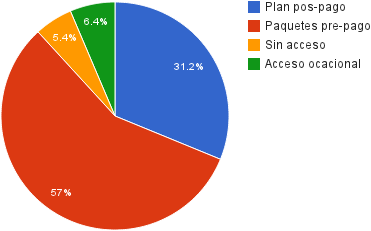
\includegraphics[scale=0.8]{resultados/imagenes/ubicacion_acceso_internet.png}
\caption{Acceso a internet desde dispositivos móviles}
\label{fig:ubicacion_acceso_internet}
\end{figure}

Por otro lado, en la figura\ref{fig:ubicacion_sistemas_operativos} se muestra los sistemas 
operativos móviles utilizados por los usuarios encuestados. Se puede observar que Android 
lidera con un $61.3\%$, le sigue Windows Phone con un $12.9\%$.

\begin{figure}[ht!]
\centering
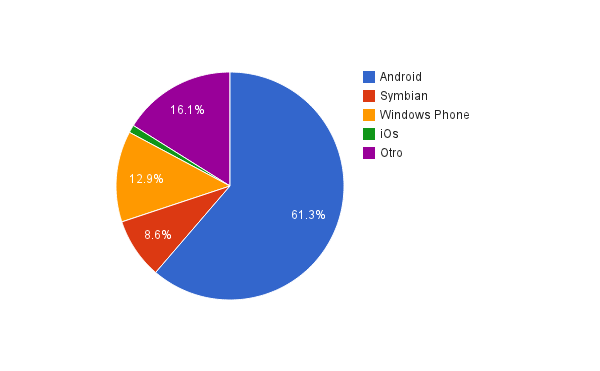
\includegraphics[scale=0.8]{resultados/imagenes/ubicacion_sistemas_operativos.png}
\caption{Sistemas operativos móviles utilizados}
\label{fig:ubicacion_sistemas_operativos}
\end{figure}

Por último, se discrimina a los encuestados para determinar cuantos de ellos tiene dispositivos
móviles que cumplen los requisitos mínimos para utilizar la solución propuesta según lo descripto
en la sección \ref{sec:ubicacion}. En la figura \ref{fig:ubicacion_requisitos_minimos} se puede 
observar que el $18,3\%$ de los encuestados cumplen con los requisitos.

\begin{figure}[ht!]
\centering
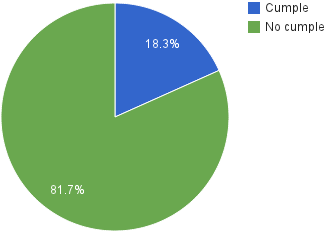
\includegraphics[scale=0.8]{resultados/imagenes/ubicacion_requisitos_minimos.png}
\caption{Dispositivos que cumplen con los requisitos mínimos para la prueba}
\label{fig:ubicacion_requisitos_minimos}
\end{figure}